\documentclass{beamer}

\usepackage{graphicx}
\usepackage{amsmath}

\begin{document}
\title{Public Key Crypto \& Digital Certificates}
\author{Hollie Baker}
\date{Dev Lunch August 2019}

\frame{\titlepage}

\frame{
    \frametitle{Alice and Bob need to talk, but they are being watched...}

    They need to encrypt their communications, but they don't have a secure channel to share an \em{encryption key}.

    One option is to use the \em{RSA cryptosystem}.
}

\frame{
    \title{Rivest, Shamir \& Adleman}

    \begin{center}
        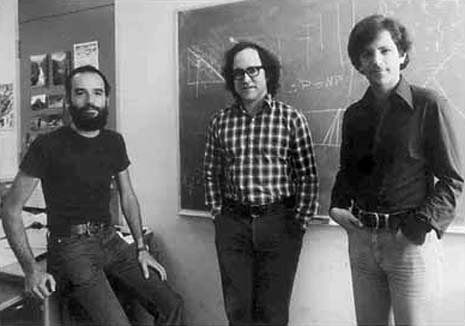
\includegraphics[width=.5\textwidth]{rsa}
    \end{center}
}

\frame{
    \frametitle{Rivest, Shamir \& Adleman}

    The original idea of public key crypto was published by Diffie and Hellman in 1976, but they left the implementation as an open question.

    Rivest, Shamir and Adelman, three MIT academics, started working on it in the 1990s.

    Rivest and Shamir were computer scientists, and as such they proposed lost of ideas.

    Meanwhile it fell to Adelman, a mathematician, to find vulnerabilities in their potential functions.
}

\frame{
    \frametitle{Rivest, Shamir \& Adelman}

    The breakthrough happened one night in April 1987 after a student party.

    Rivest, drunk and unable to sleep, started reading a maths textbook on the sofa.

    He begun thinking about the problem, and had the famous RSA one-way function formulated by the morning.

    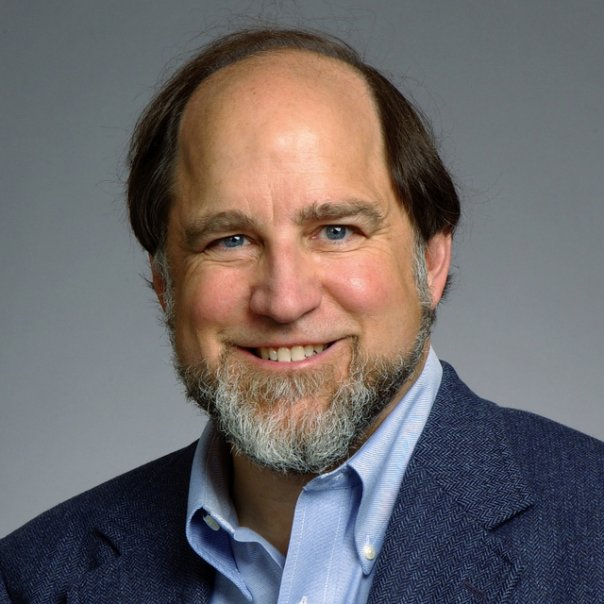
\includegraphics{Ronald_L_Rivest_photo}
}

\frame{
    \frametitle{Clifford Cocks}

    Meanwhile, in the 1970s at GCHQ, Clifford Cocks was working on the same problem.

    He developed an equivalent system, but it was kept classified until RSA was published in 1997.

    As far as we know, it was never deployed because of the cost of computational power at the time.

    \includegraphics{Clifford-Cocks-FRS}
}

\frame{
    \frametitle{The RSA Cryptosystem}

    \begin{center}
        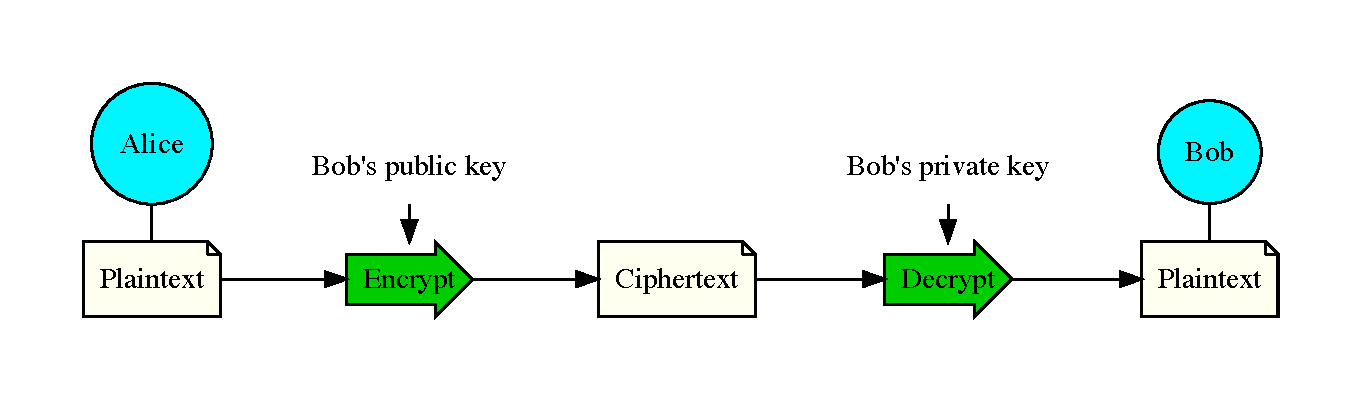
\includegraphics{pkc}
    \end{center}

    Bob’s key consists of two parts: public part which he publishes, and a private part which he keeps secret.

    The idea is that anyone can encrypt with the public key, but only Bob can decrypt with his private key.
}

\frame{
    \title{RSA: Maths Background}

    RSA relies on Euler's phi function.

    $$
    \phi(n) = \text{the number of integers } 1\le b \le n \text{ such that } GCD(b,n)=1
    $$

    Note: $GCD(b,n)$ means the greatest common divisor or $b$ and $n$.

    In other words, $\phi(n)$ is the number of integers $\le n$ which are relatively prime with $n$.
}

\frame{
    \frametitle{RSA: Maths Background}

    Two important properties of Euler's phi function are
    \begin{enumerate}
        \item If $p$ is a prime number, then $\phi(p) = p-1$.
        \item If $p$ and $q$ are relatively prime, then $\phi$ is multiplicative - i.e.,
        $$
        \phi(pq) = \phi(p)\phi(q).
        $$
    \end{enumerate}
}

\frame{
    \frametitle{RSA: Maths Background}

    RSA makes use of modular arithmetic.

    $$a \mod n$$

    Is the remainder of $a$ divided by $n$.
}

\frame{
    \frametitle{RSA: Maths Background}

    We also need ``congruence modulo $n$''

    Two integers $a$ and $b$ are congruent modulo $n$, written

    $$a \equiv b \mod n$$

    if $a - b$ is divisible by $n$.

    You could also think of it as
    $$
    (a \mod n) = (b \mod n).
    $$
}

\frame{
    \frametitle{RSA: Key Generation}

    \begin{itemize}
        \item Pick two \em{large, prime integers} $p$ and $q$.
        \item Calculate
        $$
        n = pq.
        $$
        \item Calculate $\phi(n)$. This is easy because we know $p$ and $q$ which are prime, and because $\phi$ is multiplicative. I.e.,
        $$
        \phi(pq) = \phi(p)\phi(q) = (p-1)(q-1).
        $$
        \item Choose $e$ such that $e$ is relatively prime with $\phi(n)$. \em{Publish $e$, it will be the encryption exponent.}
        \item Find $d$, the multiplicative inverse of $e \mod n$. This can be done efficiently using a well-known GCD algorithm (called the Extended Euclidean Algorithm).
        \em{Keep $d$ secret. It will be the decryption exponent.}
    \end{itemize}

    $p$, $q$ and $d$ have to be kept secret. $d$ because it's the decryption exponent, and $p$ and $q$ because, given $e$ which is public, anyone can quickly work out $d$.
}

\frame{
    \frametitle{RSA: Encryption and Decryption}

    Encryption and decryption works by raising a number, the plaintext, to a power modulo $n$.

    The encryption function is
    $$
    C = P^e \mod n.
    $$

    The decryption function is
    $$
    P = C^d \mod p.
    $$

    Decryption is the inverse of encryption, i.e.,
    $$
    P \equiv P^{ed} \mod n.
    $$
    You can prove it with number theory stuff like Fermat's Little theorem, and this is why RSA works.
}

\frame{
    \frametitle{RSA: Security}

    RSA is secure because factorising large integers is \em{hard}.

    For an attacker to break RSA with only the public information, $e$ and $n$, she needs to find $\phi(n)$. There are two options
    \begin{itemize}
        \item Factorise $n$ to find the prime numbers $p$ and $q$ and then calculate $\phi(n) = \phi(pq)$ - \em{hard}
        \item Find $\phi(n)$ directly with only $n$ to work with - \em{there's no known algorithm for that either.}
    \end{itemize}

    The RSA Factoring challenge gave prizes for people who could factor large numbers.

    The RSA problem asks ``given $C=P^e \mid n$, $e$ and $n$, what's $P$?'' It's one of those famous unsolved computer science problems.

    But maths is hard, so attackers often resort to a man-in-the-middle attack.
}

\frame{
    \frametitle{RSA: In practice}

    Basic RSA has some issues...
    \begin{itemize}
        \item {\bf Small exponents}: If $C = P^e \mod n$ is less than $n$, you just take the $e$-th root of $C$ - no modular arithmetic to worry about.
        \item \textbf{Broadcast Attacks}: If the same plaintext is sent using the same encryption exponent but different moduluses $n$, the Chinese remainder theorem can be used to decrypt the message. Hastad extended this attack, and Coppersmith built on that.
        \item \textbf{RSA encryption is multiplicative}: $(P_1 P_2)^e\mod n \equiv P_1^e P_2^e \mod n$. This opens up chosen plaintext attack possibilities.
    \end{itemize}

    The solution is to add structured, randomised padding, for example the OAEP (Optimal Asymmetric Encryption Padding) is used in practice.
}

\frame{
    \frametitle{Bob receives a message and needs to verify that it really came from Alice}

    The solution is for Alice to sign the message to create a digital signature, and send this to Bob for him to verify.
}
\frame{
    \frametitle{Digital Signatures}

    \begin{center}
        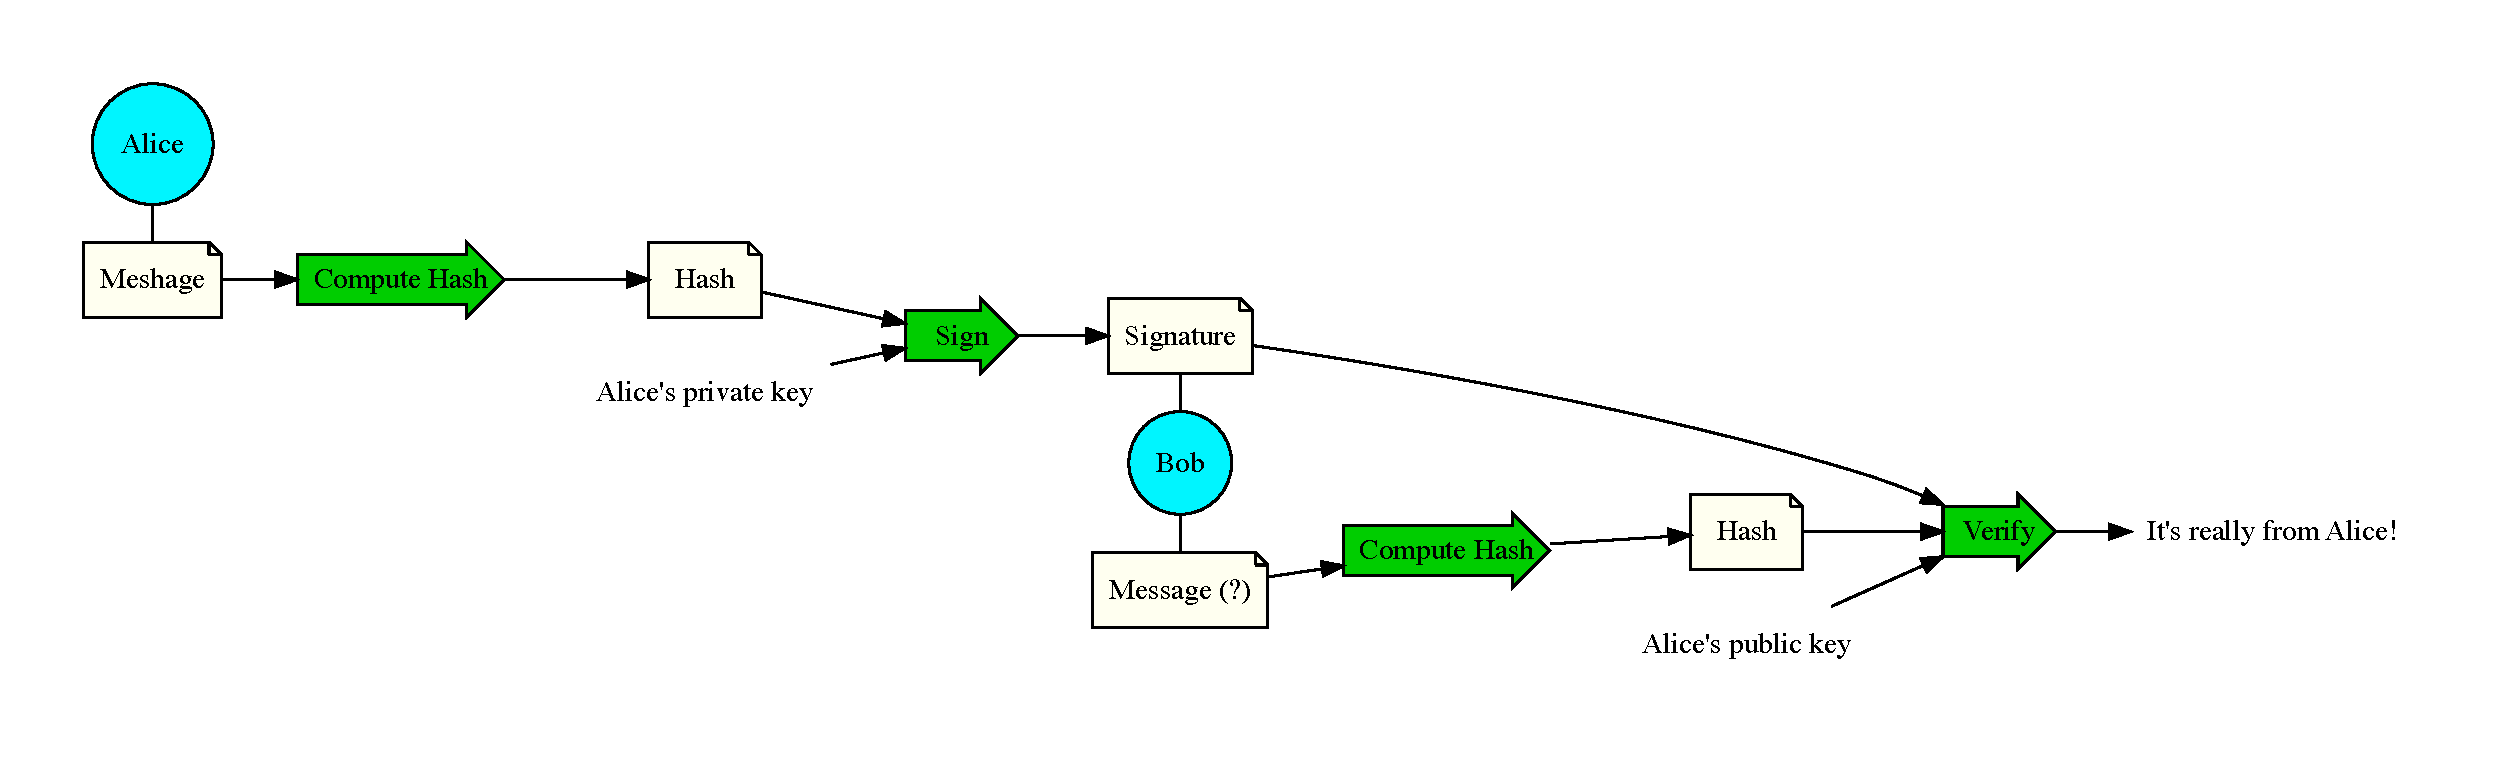
\includegraphics[width=\textwidth]{sig}
    \end{center}

    Only Alice can create this particular signature because only she has the private key. On the other hand, anybody can verify the message using Alice's public key.

    Before signing, the message must be hashed. This is to help prevent ``forgeries'' - messages that appear to be from Alice, but really aren't.
}

\frame{
    \frametitle{Digital Certificates}

    Digital signatures provide authentication by linking a public key to it's owner.

    They contain the public key, along with a digital signature of the public key - for verifying that the public key has not been tampered with. Digital certificates also contain details of it's owner and some metadata about the certificate itself.
}

\frame{
    \frametitle{But how do we know the certificate is for real}

    This is where the Certificate Authority (CA) comes in. A CA is a trusted entity who is responsible for issuing and revoking certificates. To get a certificate, you have to prove to the CA that you are who you say you are. E.g., if you want an SSL certificate for a certain domain, you have to show that you own that domain.

    Often the process of checking an entity is legit is outsourced to a Registration Authority (RA) who does all the necessary checks and then lets the CA know if the entity can be trusted so a certificate can be issued.

    Certificates can also be revoked, e.g., if it turns out the entity can't be trusted after all. This is managed by the CA, who keep a list of revoked certificates which the user must check against.

    CA's can be arranged in a hierarchy, with a ``root CA'' at the top, who are really trustworthy and all the other CA's look up to it.
}

\frame{
    \begin{center}
        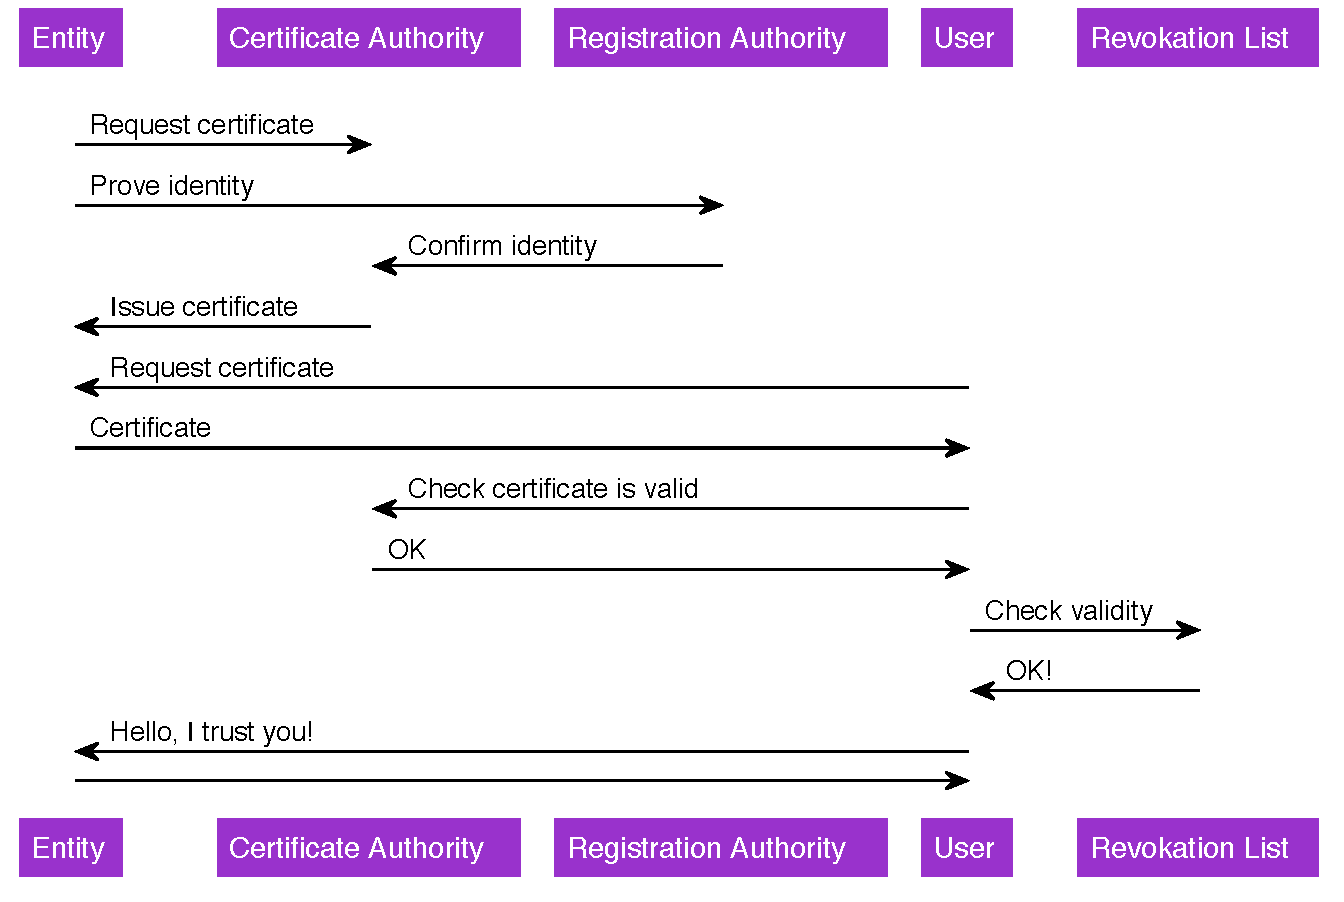
\includegraphics[width=\textwidth]{ca-sequence.pdf}
    \end{center}
}
\end{document}
